\subsection{Темпоральна медіана}

Введемо необхідні означення.

\begin{definition}
    Накопичувальна сума масиву \cite{bib:integral_image} $X$~---~це масив, кожний елемент якого є сумою всіх попередніх.
\end{definition}

Наведемо рекурентну формулу обчислення накопичувальної суми
\begin{equation}
    S_1 = a_1, \qquad S_n = a_n + S_{n-1}.
    \label{eq:summed_table_formula}
\end{equation}

\begin{definition}
    Медіаною \cite{bib:median_in_statistics} називають елемент, який стоїть посередині впорядкованого масиву.
    Якщо кількість елементів парна, то медіаною називається середнє значення між двома числами,
    що стоять посередині масиву.
\end{definition}

\begin{definition}
    Темпоральною медіаною у комп'ютерному зорі називають зображення,
    в кожному пікселі якого знаходиться медіанне значення, що знайдене між значеннями пікселів у часовому проміжку
    (рис. \ref{fig:temporal_median_example}).
\end{definition}

Темпоральну медіану застосовують у комп'ютерному зорі для отримання
фону сцени у відео \cite{bib:temporal_median_example}.
Тобто всі об'єкти, що рухаються, зникають на медіанному зображенні
(рис. \ref{fig:temporal_median_example}).
Розрахунок темпоральної медіани складається з наступних кроків:
\begin{enumerate}
    \item береться набір кадрів деякого часовому проміжку;
    \item сортуємо по кожному пікселю масиви;
    \item беремо медіану також по кожному пікселю.
\end{enumerate}

\begin{figure}[H]
    \centering
    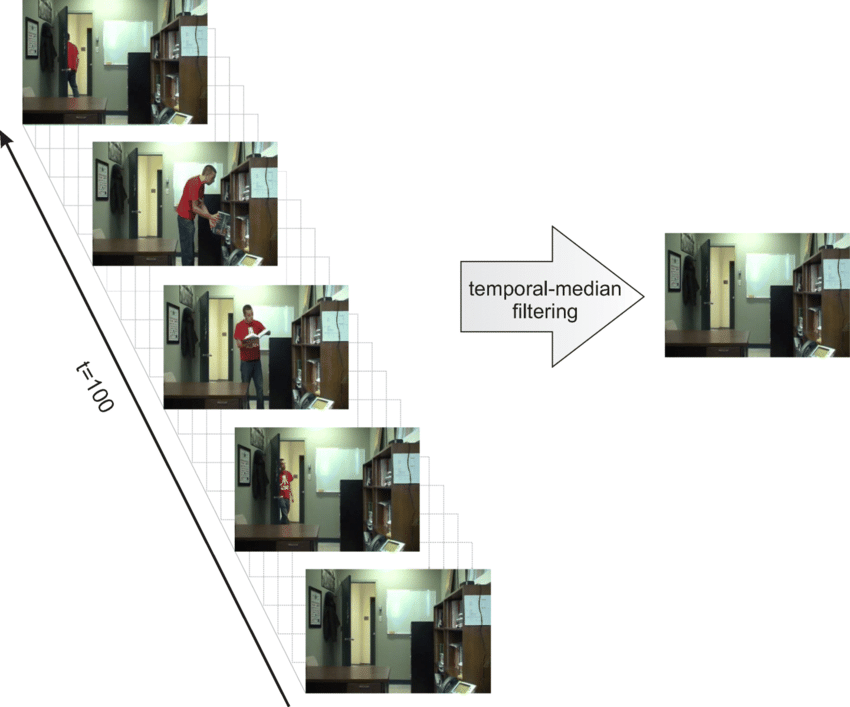
\includegraphics[width=0.5\textwidth]{images/temporal_median_example_1}
    \caption{Приклад отримання фону без людини шляхом використання темпоральної медіани
        \cite{bib:temporal_median_example}
        \label{fig:temporal_median_example}
    }
\end{figure}
Даний метод можна застосовувати як для прибирання швидких рухомих об'єктів,
так і для  отримання зображення із високою роздільною здатністю (super-resolution).

\subsection{Швидка медіана для зображень}

Розглянемо простий випадок взяття медіани.
Нехай у нас є не відсортований масив цілих чисел з множини $\{0,..., 255\}$.
Для того, щоб знайти в ньому медіану, потрібно відсортувати масив.
Для сортування масиву можна використати алгоритм швидкого сортування (quick sort)
\cite{bib:quick_sort}. У середньому випадку він працює за $\mathcal{O}(n\log{}n)$, в
найгіршому $\mathcal{O}(n^2)$.
Запропонований нижче алгоритм працюватиме за $\mathcal{O}(n)$.

Використаємо гістограму як хеш-таблицю  значень від $0$ до $255$.
\begin{definition}
    Хеш-таблиця ~---~ це структура з елементом \textit{{ключ: значення}}, де
    ключ є унікальним ідентифікатором.
\end{definition}

\begin{definition}
    Гістограма зображення $I$ ~---~ це масив, в якому елемент під індексом $i$ містить число, що показує скільки
    разів у зображенні $I$ зустрічається значення $i$.
\end{definition}

Позиція елемента $i$ в гістограмі є значенням піксела, а значення елемента на позиції $i$ ~---~ це
кількість повторень $i$ на самому зображенні $I$.

Введемо операції
\begin{itemize}
    \item $A[i]$ ~---~ взяття елемента в масиві $A$ під номером $i$;
    \item $A[i:j]$ ~---~ взяття підмасиву масиву $A$, починаючи включно з елементу $i$ до $j$ не включно;
    \item $a \mod b$ ~---~ взяття остачі від ділення числа $a$ на $b$;
    \item $\left\lceil a \right\rceil$ ~---~ округлення дійсного числа $a$ до верхньої границі;
    \item $\left\lfloor a \right\rfloor$ ~---~ округлення дійсного числа $a$ до нижньої границі;
    \item $\overline{a,b}$ ~---~ множина цілих чисел на відрізку від $a$ до $b-1$, якщо $a \le b$,
          інакше  ~---~ від $b-1$ до $a$.
\end{itemize}
Наведемо алгоритм \ref{al:median_hash} знаходження медіани в одновимірному випадку.

\begin{algorithm}[H]
    \caption{Знаходження медіани для одновимірного масиву з хеш-таблицею.}
    \label{al:median_hash}
    \begin{algorithmic}
        \State \textbf{Вхід:} не відсортований масив $A$, $\ell$ ~---~ кількість елементів.
        \State \textbf{Вихід:} $m$ ~---~ медіанне значення масиву $A$.
        \State \textbf{Ініціалізація:} $H$ ~---~ цілочисельний масив, що заповнено нулями (гістограма) на $256$ елементів.
        \State \textbf{Крок 1:} Заповнюємо масив $H$.
        \State $\forall a \in A$
        \State \qquad $ H[a] \gets H[a] + 1 $
        \State \textbf{Крок 2:} Сортуємо масив $ A $:
        \State $ i \gets 0 $
        \State $ \forall j \in \overline{0,256} $
        \State \qquad  $ A[i:i+H[j]] \gets j $
        \State \qquad  $ i \gets i + H[j] $
        \State \textbf{Крок 3:} Знаходимо $m = \frac{A[  \left\lfloor \ell/2 \right\rfloor   ] + A[\left\lceil \ell/2 \right\rceil ]}{2} $
    \end{algorithmic}
\end{algorithm}

\subsection{Побудова швидкої медіани для зображень}

Нехай у нас на вхід подається черга із $m$ картинок. Кожну ітерацію приходить нова картинка.
\begin{figure}[H]
    \centering
    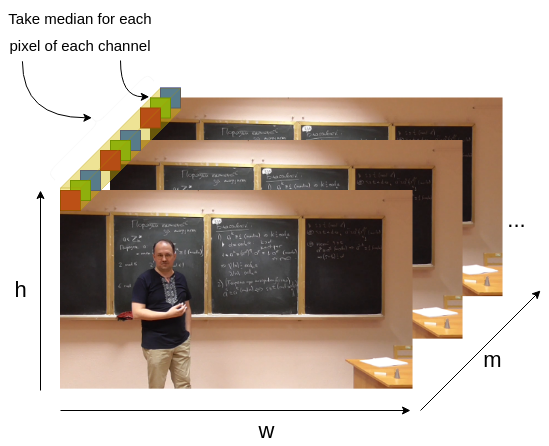
\includegraphics[width=0.6\textwidth]{images/median_seq}
    \caption{Приклад послідовності картинок для формування медіани з відео \cite{video:mmzi:yakovlev_numbers_theory}
        \label{fig:median_seq_example}
    }
\end{figure}
Для простішого пояснення методу швидкої медіани візьмемо одноканальне зображення
зображення у відтінках сірого розмірами $h \times w$, де $h$ ~---~ висота, $w$ ~---~ ширина,
але в реальності операції, що наведені нижче виконуються для трьохканального $RGB$ зображення
окремо для кожного каналу.

В інформаційній технології перетворення відеозапису з дошки у слайд-шоу
\cite{bib:creating_slides_1} \cite{bib:patent_board}
алгоритм швидкої медіани застосовується на панорамних знімках
з метою знешумлення на підвищення якості написів на дошці.

Введемо такі масиви:
\begin{itemize}
    \item $F$~---~масив із $n$ зображень із відео або панорамних знімків, розміром $n \times  h \times w$;
    \item $S$~---~масив, що містить  всі $m$ вхідних зображень розміром $h \times w \times m$;
    \item $M$~---~масив, що є темпоральною медіаною по $m$ зображень розміром $h \times w$;
    \item $C$~---~масив, що є накопичувальною сумою розміром $h \times w \times 256$. У кожному елементі під індексом $i$ в
          масиві з $256$ елементів зберігається число, що означає кількість разів присутності значення $i$ в кожному
          масиві з $m$ елементів в масиві $S$.
\end{itemize}

Розглянемо алгоритм ініціалізації масивів $S, M, C$ (алгоритм \ref{al:init_s_m_c}).
\begin{algorithm}[H]
    \caption{Алгоритм ініціалізації масивів $S, M, C$}
    \label{al:init_s_m_c}
    \begin{algorithmic}
        \State \textbf{Вхід:} $m$ ~---~ кількість зображень для обчислення медіани,
        $I$ ~---~ перше зображення з відео.
        \State \textbf{Вихід:} масиви $S, M, C$.
        \State \textbf{Крок 1:} Створюємо $S$ шляхом конкатенації $m$ разів масиву $I$.
        Тоді $S$ має розміри $h \times w \times m$. Тобто зараз у $S$ міститься
        $m$ копій зображення $I$.
        \State \textbf{Крок 2:} Створюємо медіанне зображення: $M \gets I$
        \State \textbf{Крок 3:} Створюємо нульовий масив $C$ розмірами $h \times w \times 256$.
        \State \textbf{Крок 4:} Заповнюємо $C$ використовуючи $M$:
        \State $\forall i \in \overline{0,h}$
        \State \qquad $\forall j \in \overline{0,w}$
        \State \qquad \qquad $C[i,j,M[i,j]] \gets m$
        \State \textbf{Крок 5:} Обраховуємо накопичувальну суму $E$ для кожного масиву з $256$ елементів
        масиву $C$ по формулі \eqref{eq:summed_table_formula}.
        \State \textbf{Крок 6:} $C \gets E$.
    \end{algorithmic}
\end{algorithm}

Наведемо алгоритм оновлення $C$ (алгоритм \ref{al:update_C}) по двом зображенням,
одне з яких назвемо інкрементним $I_{in}$, а інше декрементним $I_{de}$.

\begin{algorithm}[H]
    \caption{Алгоритм оновлення $C$}
    \label{al:update_C}
    \begin{algorithmic}
        \State \textbf{Вхід:} масив $C$, інкрементне та декрементне зображення $I_{in}, I_{de}$.
        \State \textbf{Вихід:} оновлений масив $C$.
        \State $\forall i \in \overline{0,h}$
        \State \qquad  $\forall j \in \overline{0,w}$
        \State \qquad \qquad $\forall k \in \overline{I_{in}[i,j],256}$
        \State \qquad \qquad \qquad $C[i,j,k] \gets C[i,j,k] + 1$
        \State \qquad \qquad $\forall k \in \overline{I_{de}[i,j],256}$
        \State \qquad \qquad \qquad $C[i,j,k] \gets C[i,j,k] - 1$
    \end{algorithmic}
\end{algorithm}

Також потрібен алгоритм оновлення медіанного зображення (алгоритм \ref{al:update_M}) $M$.

\begin{algorithm}[H]
    \caption{Алгоритм оновлення $M$}
    \label{al:update_M}
    \begin{algorithmic}
        \State \textbf{Вхід:} масиви $M, S, C$, та параметр $m$.
        \State \textbf{Вихід:} оновлений масив $M$.
        \State $p \gets \left\lfloor m/2 \right\rfloor$ \Comment{припускаємо, що медіана знаходиться посередині}
        \State $\forall i \in \overline{0,h}$
        \State \qquad  $\forall j \in \overline{0,w}$
        \State \qquad \qquad  Якщо $C[i,j, M[i,j]] \geq p$:
        \State \qquad \qquad \qquad $\forall k \in \overline{M[i,j]-1,-1}$
        \State \qquad \qquad \qquad \qquad  Якщо $C[i,j,k] \leq p$:
        \State \qquad \qquad \qquad \qquad \qquad $p_{new} \gets C[i,j,k+1]$
        \State \qquad \qquad \qquad \qquad \qquad стоп
        \State \qquad \qquad інакше:
        \State \qquad \qquad \qquad $\forall k \in \overline{M[i,j]+1,256}$
        \State \qquad \qquad \qquad \qquad  Якщо $C[i,j,k] \geq p$:
        \State \qquad \qquad \qquad \qquad \qquad $p_{new} \gets C[i,j,k-1]$
        \State \qquad \qquad \qquad \qquad \qquad стоп
        \State \qquad \qquad $M[i,j] \gets S[i,j, \left\lfloor p_{new}\right\rfloor ]$
    \end{algorithmic}
\end{algorithm}

Використовуючи вищенаведені алгоритми,
можна записати сам метод швидкої медіани для потоку зображень (алгоритм \ref{al:fast_median_algorithm}).

\begin{algorithm}[H]
    \caption{Алгоритм швидкої медіани для потоку зображень}
    \label{al:fast_median_algorithm}
    \begin{algorithmic}
        \State \textbf{Вхід:} масив $F$, та параметр $m$.
        \State \textbf{Вихід:} список медіан $L$.
        \State \textbf{Крок 1:} Ініціалізуємо масиви $S, M, C$ по зображенню $F[1]$ по алгоритму \ref{al:init_s_m_c}
        \State \textbf{Крок 2:} $q \gets 0$ \Comment{лічильник черги}
        \State  $\forall i \in \overline{0,n-1}$
        \State \qquad \textbf{Крок 3:} Оновлюємо $C$ по алгоритму \ref{al:update_C} з параметрами $C$,
        $F[i]$ ~---~ інкрементне зображення, $F[i+1]$ ~---~ декрементне зображення.
        \State \qquad \textbf{Крок 4:} Оновлюємо $M$ по алгоритму \ref{al:update_M} з параметрами $C, M, m$.
        \State \qquad \textbf{Крок 5:} Ставимо на місце $q$ в масиві $S$ зображення $F[i]$
        \State \qquad \textbf{Крок 6:} Оновлюємо лічильник $q \gets (q+1) \mod m$
        \State \qquad \textbf{Крок 7:} Додаємо нову $M$ у $L$.
    \end{algorithmic}
\end{algorithm}

Для аналогії наведемо звичайний алгоритм \ref{al:temporal_median} медіани для $S$.
\begin{algorithm}[H]
    \caption{Звичайний алгоритм медіани для $S$}
    \label{al:temporal_median}
    \begin{algorithmic}
        \State \textbf{Вхід:} масив $S$, та параметр $m$.
        \State \textbf{Вихід:} масив $M$.
        \State  $\forall i \in \overline{0,h}$
        \State \qquad  $\forall i \in \overline{0,w}$
        \State \qquad \qquad  Сортуємо масив з $m$ елементів і позначимо за $e$.
        \State \qquad \qquad  $M[i,j] \gets e[\left\lfloor m/2 \right\rfloor ]$ \Comment{записуємо значення медіани}
    \end{algorithmic}
\end{algorithm}

\subsection{Порівняння складності}
Обчислимо складність швидкої медіани $m$ зображень, кожне з яких розміром $h \times w$:
$
    \mathcal{O}(h \cdot w) (\textit{ініціалізація S, M, C} )
    + \mathcal{O}(h \cdot w) (\textit{оновлення С})
    + \mathcal{O}(h \cdot w) (\textit{оновлення M}) = \mathcal{O}(h \cdot w).
$
Аналогічно для звичайного випадку із quick sort: $\mathcal{O}(h \cdot w \cdot m^2)$ у найгіршому випадку.
Варто відмітити, що таке прискорення досягається тим,
що є обмеження на використання значень від $0$ до $255$.

\clearpage
